\chapter {Tehnologii și Spațiu Virtual}

\section{Realitate virtuală}

Transpunerea în pielea diferitor personaje sau în scenarii fictive este ceva ce oamenii fac dintotdeauna. Înainte ca tehnologia să ne permită punerea pe hârtie a gândurilor și fanteziilor, ne adunam și spuneam povești, acest lucru permițându-ne să ne imaginăm pe noi înșine în fiecare din locurile descrise în poveste. Fără ajutorul tehnologiei ne puteam imagina că ne aflăm într-o altă realitate față cea în care ne găseam.

Acest lucru nu poate fi neapărat descris ca realitate virtuală în sensul în care îl folosim astăzi, dar poveștile spuse de mii de ani subliniază faptul că suntem o specie căreia îi place să își folosească mintea pentru a vizita diferite locuri, scenarii și evenimente.
Aceste caracteristici sunt ceea ce n-a împins de-a lungul secolelor să folosim tehnologia pentru a face tranziția în lumi diferite cât mai ușoară, acolo unde doar imaginația nu era de ajuns.

Folosim aceste tehnologii pentru a ne păcăli simțurile în a crede ca suntem altundeva și putem face lucruri incredibile și imposibile de realizat în viața de zi cu zi.

\subsection{Origini}

Tehnologia de \textit{simulare} a unei experiențe datează din 1929 când pionierul în aviație, Edwin Albert Link a inventat un dispozitiv numit \textit{Cutia albastră}\footnote{Original \textit{The blue box}, cunoscut și sub numele de \textit{Link Trainer}}. Era un simulator de zbor  rudimentar, echipat cu motoare pentru a simula rotația avionului pe două axe, utilizat la instruirea piloților în utilizarea comenzilor de bază. Pilotul intra în carlinga închisă izolându-se de exterior. Deși nu avea o reprezentare vizuală a unei lumi virtuale în acest simulator, folosea mișcarea artificială pentru a păcăli simțurile pilotului în a crede că se află într-un avion real.

\newpage

\begin{figure}[h]
  \centering
  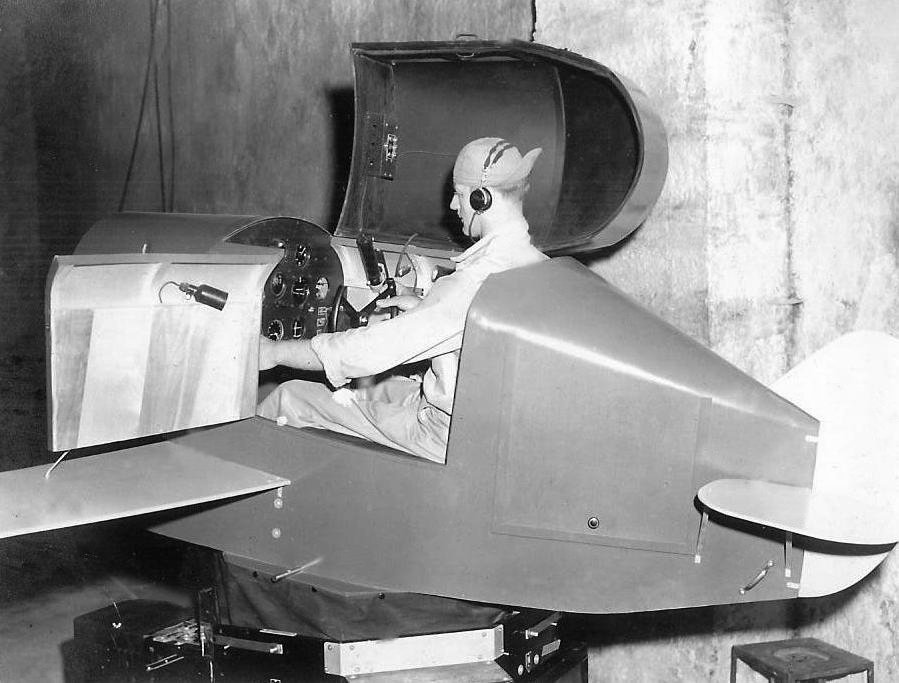
\includegraphics[scale=0.9]{img/link_trainer.jpg}
  \caption{Link Trainer, simulator de zbor inventat în 1929}
\end{figure}


Ceva mai târziu, în 1935 a fost publicată în revista științifico-fantastică \textit{Povestiri fantastice}\footnote{Original \textit{Wonder Stories}}, opera scrisă de Stanley G. Weinbaum intitulată \textit{Ochelarii lui Pygmalion}\footnote{Original \textit{Pygmalion's Spectacles}}.

Aceasta este povestea unui bărbat care primește de la un inventator o pereche de ochelari care îi permiteau purtătorului să ia parte într-o poveste ca și când ar fi cu adevărat prezent în acea lume, putând să vadă, audă, simtă, miroase și să interacționeze cu mediul înconjurător. Nu doar atât, dar purtătorul putea să vorbească personajelor iar acestea răspundeau ca și cum ar fi un alt personaj participând la acțiune.

\textit{Ochelarii lui Pygmalion} este prima mențiune într-o operă literară a ceea ce putem considera ca fiind realitate virtuală și se asemănă izbitor cu dispozitivele VR disponibile astăzi. 
\newpage

Adevăratul pionier al realității virtuale a fost Morton Leonard Heilig, care utilizându-și experiența cinematografică a dezvoltat într-o perioadă de mai mulți ani un aparat numit \textit{Sensorama}, început în 1957 și patentat în 1962.
Sensorama era construit ca jocurile de tip arcade ale anilor '80. Oferea utilizatorului experiența de-a conduce o motocicletă pe străzile din Brooklyn, putea simți vântul pe față, vibrațiile scaunului motocicletei, viziune tridimensională și chiar mirosul orașului.
Heilig a filmat o serie de filme pentru invenția sa, dar din nefericire nu a avut parte de finanțarea necesară pentru Sensorama în producție.

\begin{figure}[h]
  \centering
  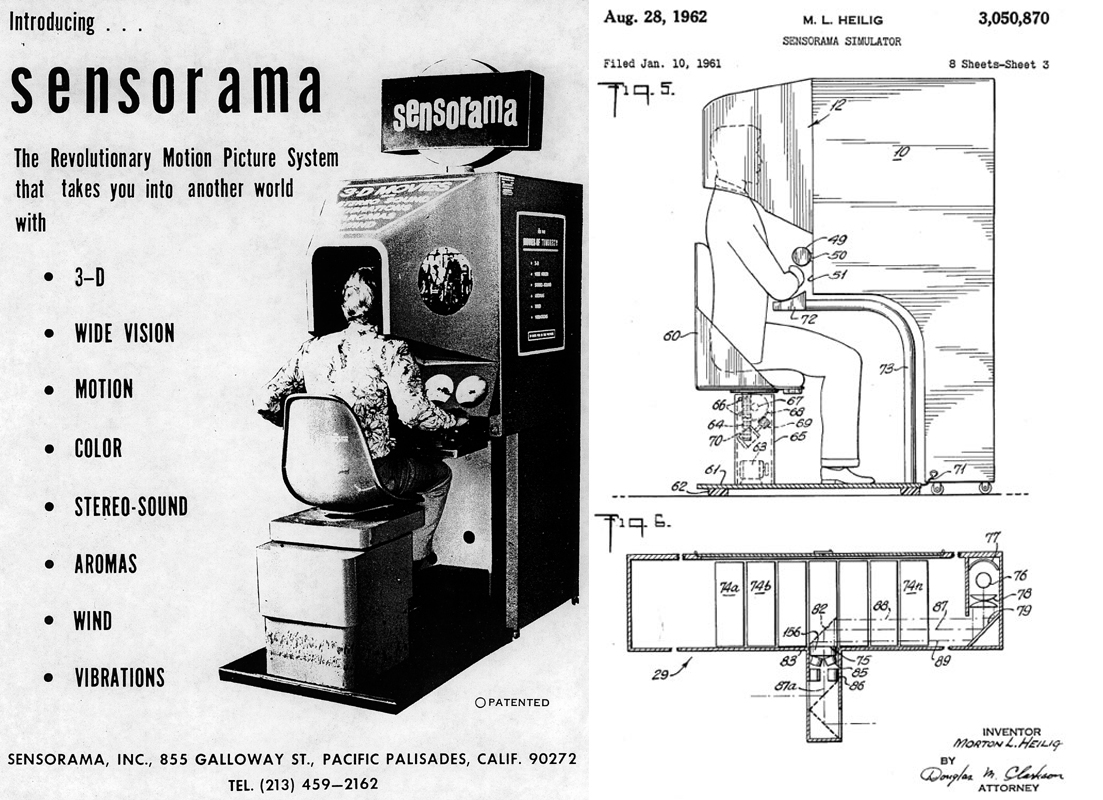
\includegraphics[scale=0.35]{img/sensorama.jpg}
  \caption{Sensorama, dezvoltat între 1957 și 1962}
\end{figure}

\subsection{Realitatea Virtuală în anii '80, '90}

Datorită înaintării progresului tehnologic, realitatea virtuală a făcut salturi uriașe în ani '80 - '90, mulțumită în special interesului dovedit de NASA în acest domeniu.

În 1985 un departament al NASA a dezvoltat \textit{Virtual Environment Display System}, o cască cu ecran stereoscopic și unghi larg de vizibilitate controlat de poziția utilizatorului, vocal și prin gesturi, cu ajutorul unor mănuși speciale.

În 1987 compania \textit{VPL} a creat o serie de tehnologii legate de VR, printre care \textit{Data Glove} și \textit{EyePhone}. VPL a fost prima companie care a comercializat căști de VR și controlere sub formă de mănuși. De asemenea Jaron Lanier fondatorul companiei este cel care a atribuit tehnologiei numele de \textit{realitate virtuală}.

La începutul anilor '90 NASA a transformat \textit{Clădirea 9} din cadrul Centrului Spațial Johnson, într-un spațiu dedicat cercetării și dezvoltării tehnologiei realității virtuale și i-au pus numele de \textit{VR lab}.
Primele căști sau HMD-uri\footnote{\textit{HMD} sau \textit{Head mounted display} este numele atribuit acestor dispozitive, neavând o traducere exactă. Traducerea \textit{ad litteram} ar fi \textit{afișaj montat pe cap} sau, mai intuitiv, \textit{cască}.} folosite de NASA la noul sediu ce cercetare în 1991, foloseau ecrane LCD cu o rezoluție de 320x240 fiind aproape de rezoluția minima a monitoarelor folosite în acea perioadă. Rezoluția acestor ecrane a crescut mult în anii următori, ca în 1994 să ajungă la 1280x1024. 

\begin{figure}[h]
  \centering
  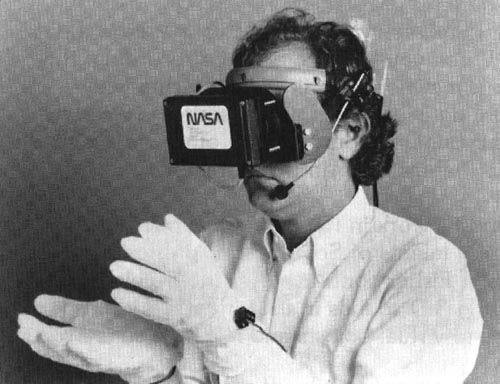
\includegraphics[scale=0.8]{img/nasaVR.jpg}
  \caption{Sistem VR dezvoltat de NASA}
\end{figure}

Una dintre activitățile în care NASA utiliza acest sistem era pentru antrenarea astronauților în folosirea costumelor \textit{EVA}\footnote{\textit{EVA} sau \textit{Extravehicular activity}, tradus ca \textit{activitate extravehiculară}, reprezintă activitățile întreținute de cosmonauți în exteriorul navetelor spațiale, și a atmosferei pământului.} în exteriorul navetelor spațiale.
În aceeași perioadă în care NASA a creat VR lab, o companie debutantă din UK, Virtuality Group a dezvoltat o serie de jocuri arcade. Principalele tipuri de jocuri comercializate erau cele menite să fie jucate din picioare și cele de tip habitaclu. Virtuality a dezvoltat primele versiuni ale elementelor ce se regăsesc în sistemele VR de astăzi, ca senzorii de detectare a mișcării în spațiu, HMD-uri cu timp de răspuns redus și alte inovații software. Căștile aveau două ecrane cu rezoluție de 276x372 și aveau un timp de răspuns de sub 50 de milisecunde.

Aceste jocuri au fost cele care au făcut publicul larg să realizeze potențialul realității virtuale.

\begin{figure}[h]
  \centering
  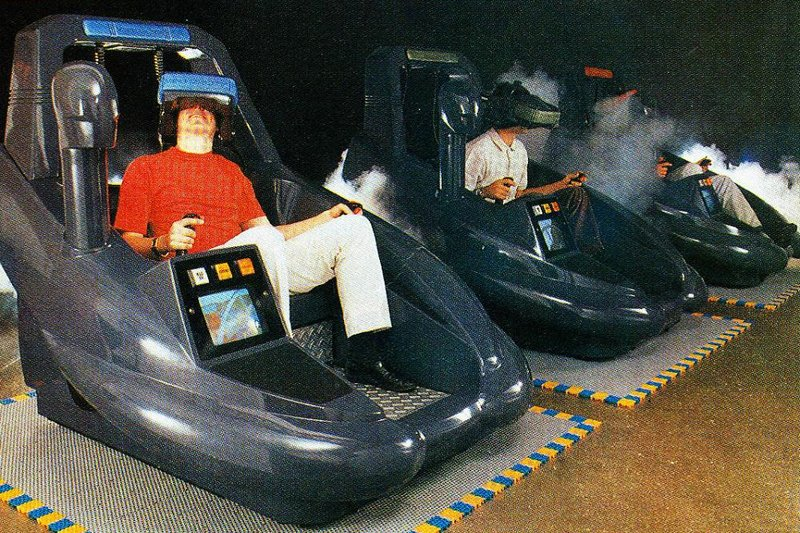
\includegraphics[scale=0.5]{img/virtuality.jpg}
  \caption{Jocuri arcade dezvoltate de Virtuality Group}
\end{figure}

Virtuality nu erau singurii din industria jocurilor interesați de realitata virtuală. SEGA a anunțat SEGA VR în 1991 deși nu a avut un prototip funcțional până în 1993 când a făcut o prezentare la o convenție de electronice. Dar din cauza unor probleme de dezvoltare și a faptului că dispozitivul provoca rău de mișcare și dureri de cap proiectul a fost anulat in 1994.
Nintendo, încercând să profite de interesul publicului pentru aceste tehnologii, a lansat \textit{Virtual boy} în 1995, care deși avea un display stereoscopic nu a fost creat pentru a putea fi purtat pe cap neavând senzori de detectare a mișcării. A fost un eșec comercial abandonat un an mai târziu. 
Un alt proiect abandonat a fost \textit{Jaguar VR,} produs de Atari în colaborare cu Virtuality, colaborare ce nu a fost sustenabilă.

Virtuality Group a continuat să-și dezvolte tehnologia printr-o colaborare cu IBM în 1995, pentru a lucra la așa numitul proiect \textit{Elysium}. Era o stație de lucru pentru PC cu aplicare în arhitectură și construcții.

Alte HMD-uri au mai fost de asemenea lansate în această perioadă, cum ar fi \textit{CyberMaxx} ce avea o serie de jocuri compatibile, ca Doom II și Duke Nukem 3D, dar vânzările au fost extrem de scăzute. \textit{i-glasses!} lansat în 1995, este un alt produs fără succes la vânzări.
\textit{VFX1} era unul dintre cele mai cunoscute astfel de produse ale perioadei, dar din nou, cu succes limitat.

Motivul din spatele eșecului acestor produse se rezumă la puterea de procesare a computerelor și consolelor, ce nu puteau oferi o experiență extraordinară. Din cauza numărului mic de cadre pe secundă combinat cu timpul mare de răspuns, acestea provocau rău de mișcare, dureri de cap și oboseala ochilor. Cu excepția câtorva fani înrăiți, interesul publicului s-a evaporat spre sfârșitul anilor '90.

\subsection{În prezent}

După o perioadă de liniște în lumea realității virtuale, telefoanele mobile au început să încorporeze touchscreen-uri care au ajutat imens la dezvoltarea ecranelor cu rezoluție mare și timp de răspuns tot mai rapid.

Palmer Luckey, antreprenorul care avea să revitalizeze VR-ul, a început ca orice adolescent fascinat de tehnologia realității virtuale colectând și adăugându-și propriile modificări vechilor HMD-uri. Prin intermediul site-ului MTBS3D\footnote{Provine de la \textit{Meant to be seen}, în traducere "trebuie să fie văzut".}, dedicat tehnologiei stereoscopice, a intrat în contact cu John Carmack\footnote{John Carmack este un celebru dezvoltator de jocuri ca, Wolfenstein 3D, Commander Keen, Doom, Quake, Rage.}, care a cerut să-i trimită un prototip.
Carmack și-a adăugat propriile modificări și a prezentat la diverse evenimente unul din primele prototipuri a ce avea sa devină \textit{Oculus Rift}.
În același timp Sony începuse să lucreze la \textit{Project Morpheus} acum cunoscut doar ca Playstation VR. Compania Valve de asemenea a devenit interesată de tehnologie iar printr-un parteneriat cu HTC au dezvoltat HMD-ul cunoscut ca \textit{HTC Vive}.

\begin{figure}[h]
  \centering
  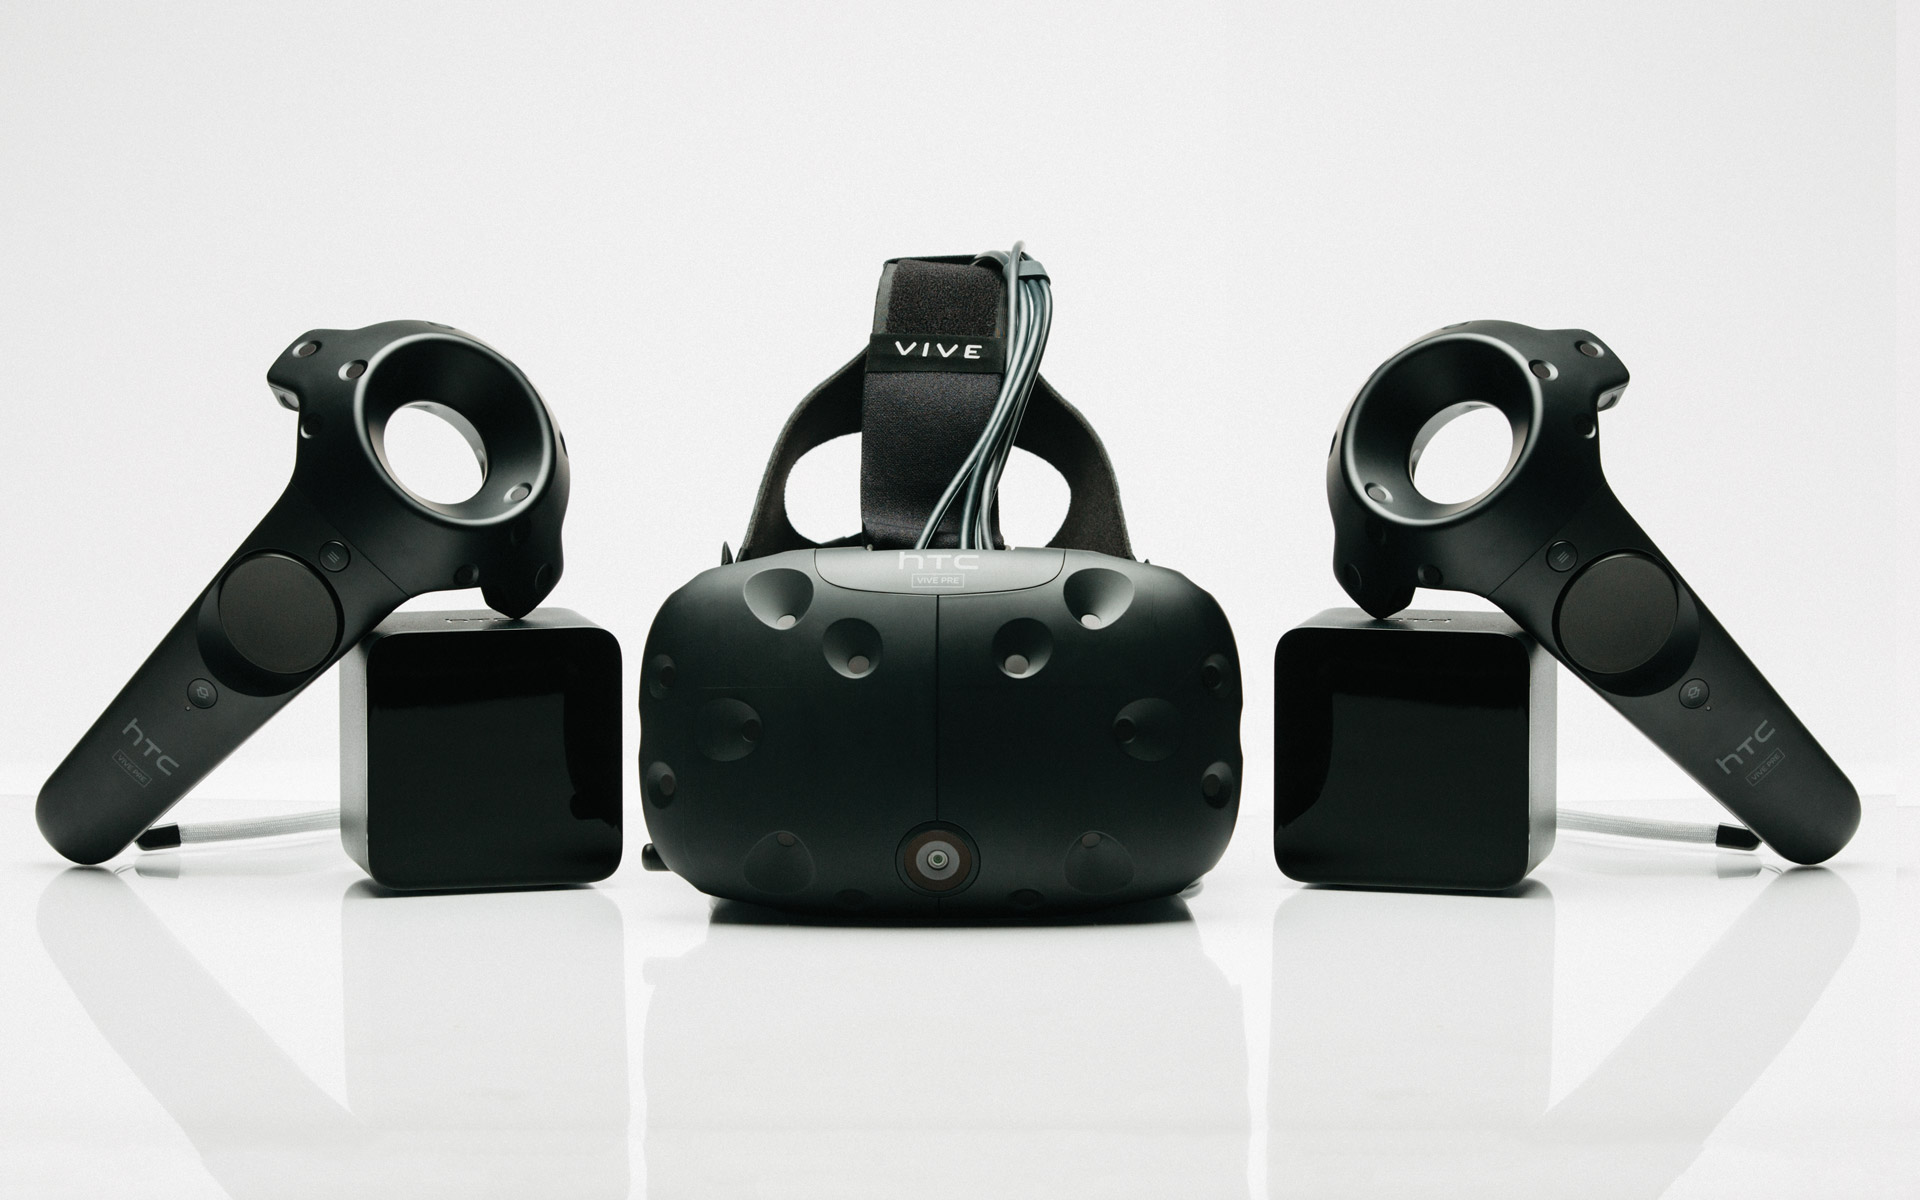
\includegraphics[scale=0.2]{img/htcvive.jpg}
  \caption{Set HTC Vive ce conține cască, controlere și senzori}
\end{figure}

În martie 2014, Facebook a cumpărat Oculus, compania fondată de Palmer Luckey, cu 2 miliarde de dolari și la scurt timp a lansat \textit{Oculus Rif DK2}\footnote{DK2 provine de la \textit{development kit} însemnând kit pentru dezvoltatori.}.

Cele două sisteme pentru PC au fost lansate la o distanță de o săptămână, pe 28 martie 2016 Oculus Rift iar pe 15 aprilie HTC Vive.
\newpage

\subsection{Oculus Rift}

\begin{figure}[h]
  \centering
  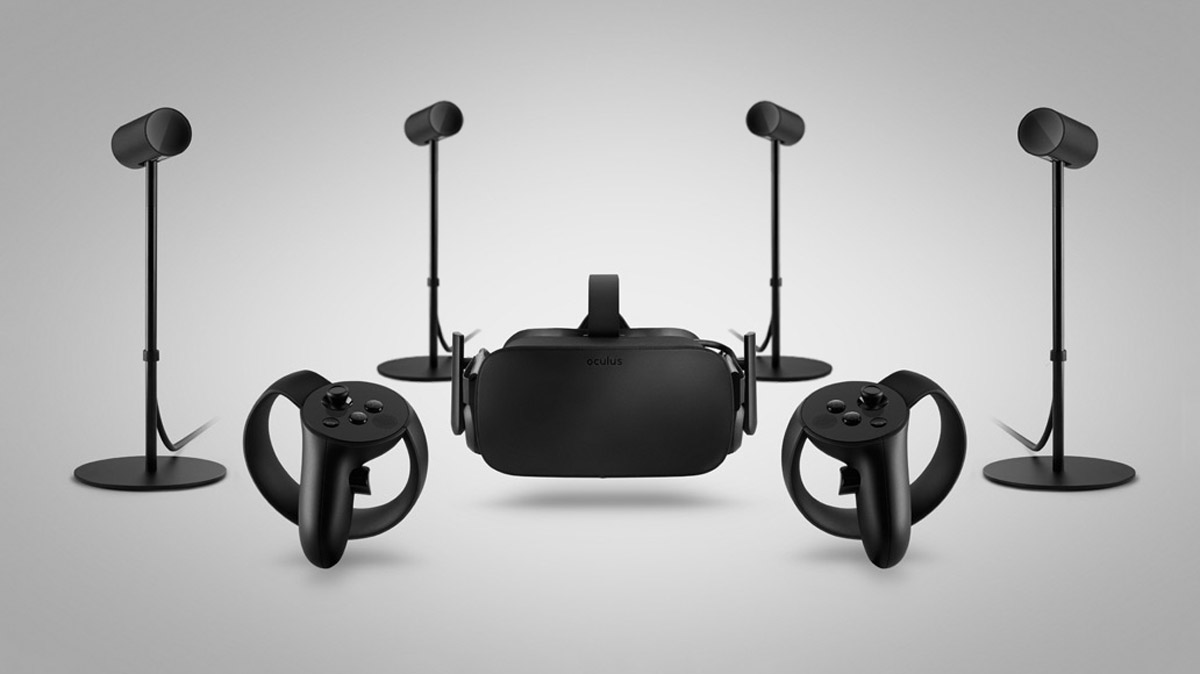
\includegraphics[scale=0.35]{img/oculusRift.jpg}
  \caption{Set Oculus Rift ce conține casca, controlere și senzori}
\end{figure}

De la lansarea campaniei pentru strângere de fonduri pe Kickstarter în 2012 unde a strâns 2,5 milioane de dolari, Oculus a scos două modele de Rift, DK1 și DK2, dedicate programatorilor, ca în martie 2016 să lanseze versiunea pentru publicul larg.
DK1 avea un ecran LCD de 7 inch (18 cm) cu o rezoluție de 1280×800 (format 16:10) ceea ce însemna o rezoluție efectivă de  640×800 pentru fiecare ochi.
DK2 a venit cu o serie de îmbunătățiri, cum ar fi, senzori de detectare a poziției, un ecran OLED cu o rezoluție de 960×1080 pentru fiecare ochi.

Oculus Rift în versiunea sa curentă are câte un ecran OLED pentru fiecare ochi, fiecare cu o rezoluție de 1080×1200, frecvență de 90Hz, și de asemenea persistență redusă, ceea ce înseamnă că afișează o imagine timp de doar 2 milisecunde pentru fiecare cadru.
Folosește lentile care asigură un câmp vizual larg. Lentilele sunt ajustabile pentru a acomoda diferite distanțe interpupilare. Această versiune are încorporată și căști cu efect audio tridimensional.

Sistemul de detectare a poziției, numit \textit{Constellation}, utilizează senzori cu infraroșu ce urmăresc dispozitivele VR. Acestea au LED-uri infraroșu în poziții cheie setate să clipească la o anumită frecvență. Astfel pot determina poziția în spațiu cu o acuratețe sub-milimetrică cu o întârziere ce tinde la zero.

Controlerele de tip \textit{Oculus Touch}, lansate mai târziu, pe 6 decembrie 2016, conțin fiecare câte două butoane trăgaci (eng. \textit{trigger}), două butoane clasice și câte un stick-analog și un sistem de detectare a mișcărilor degetelor.


\section{Prezență virtuală}

Odată intrați în lumea virtuală avem nevoie de o metodă de a putea interacționa cu noul mediu. Desigur, putem continua să folosim tastatura și mouse-ul dar asta nu are prea mult sens în cele mai multe cazuri deoarece ne restricționează libertatea de mișcare, ne afectează imersiunea, iar scopul de a interacționa cât mai natural cu elementele virtuale este complet anihilat.

Din acest motiv dezvoltatorii tehnologiilor VR împerechează HMD-urile cu controlere echipate cu senzori de mișcare, menite să simuleze prezența mâinilor în spațiul virtual, ca \textit{Oculus Touch} menționat anterior, sau \textit{Playstation Move}.
Un alt dispozitiv cu funcția de a transpune mâinile in mediul virtual, dar fără nevoia de a ține un dispozitiv fizic în mână, este \textit{Leap Motion}.

\begin{figure}[h]
  \centering
  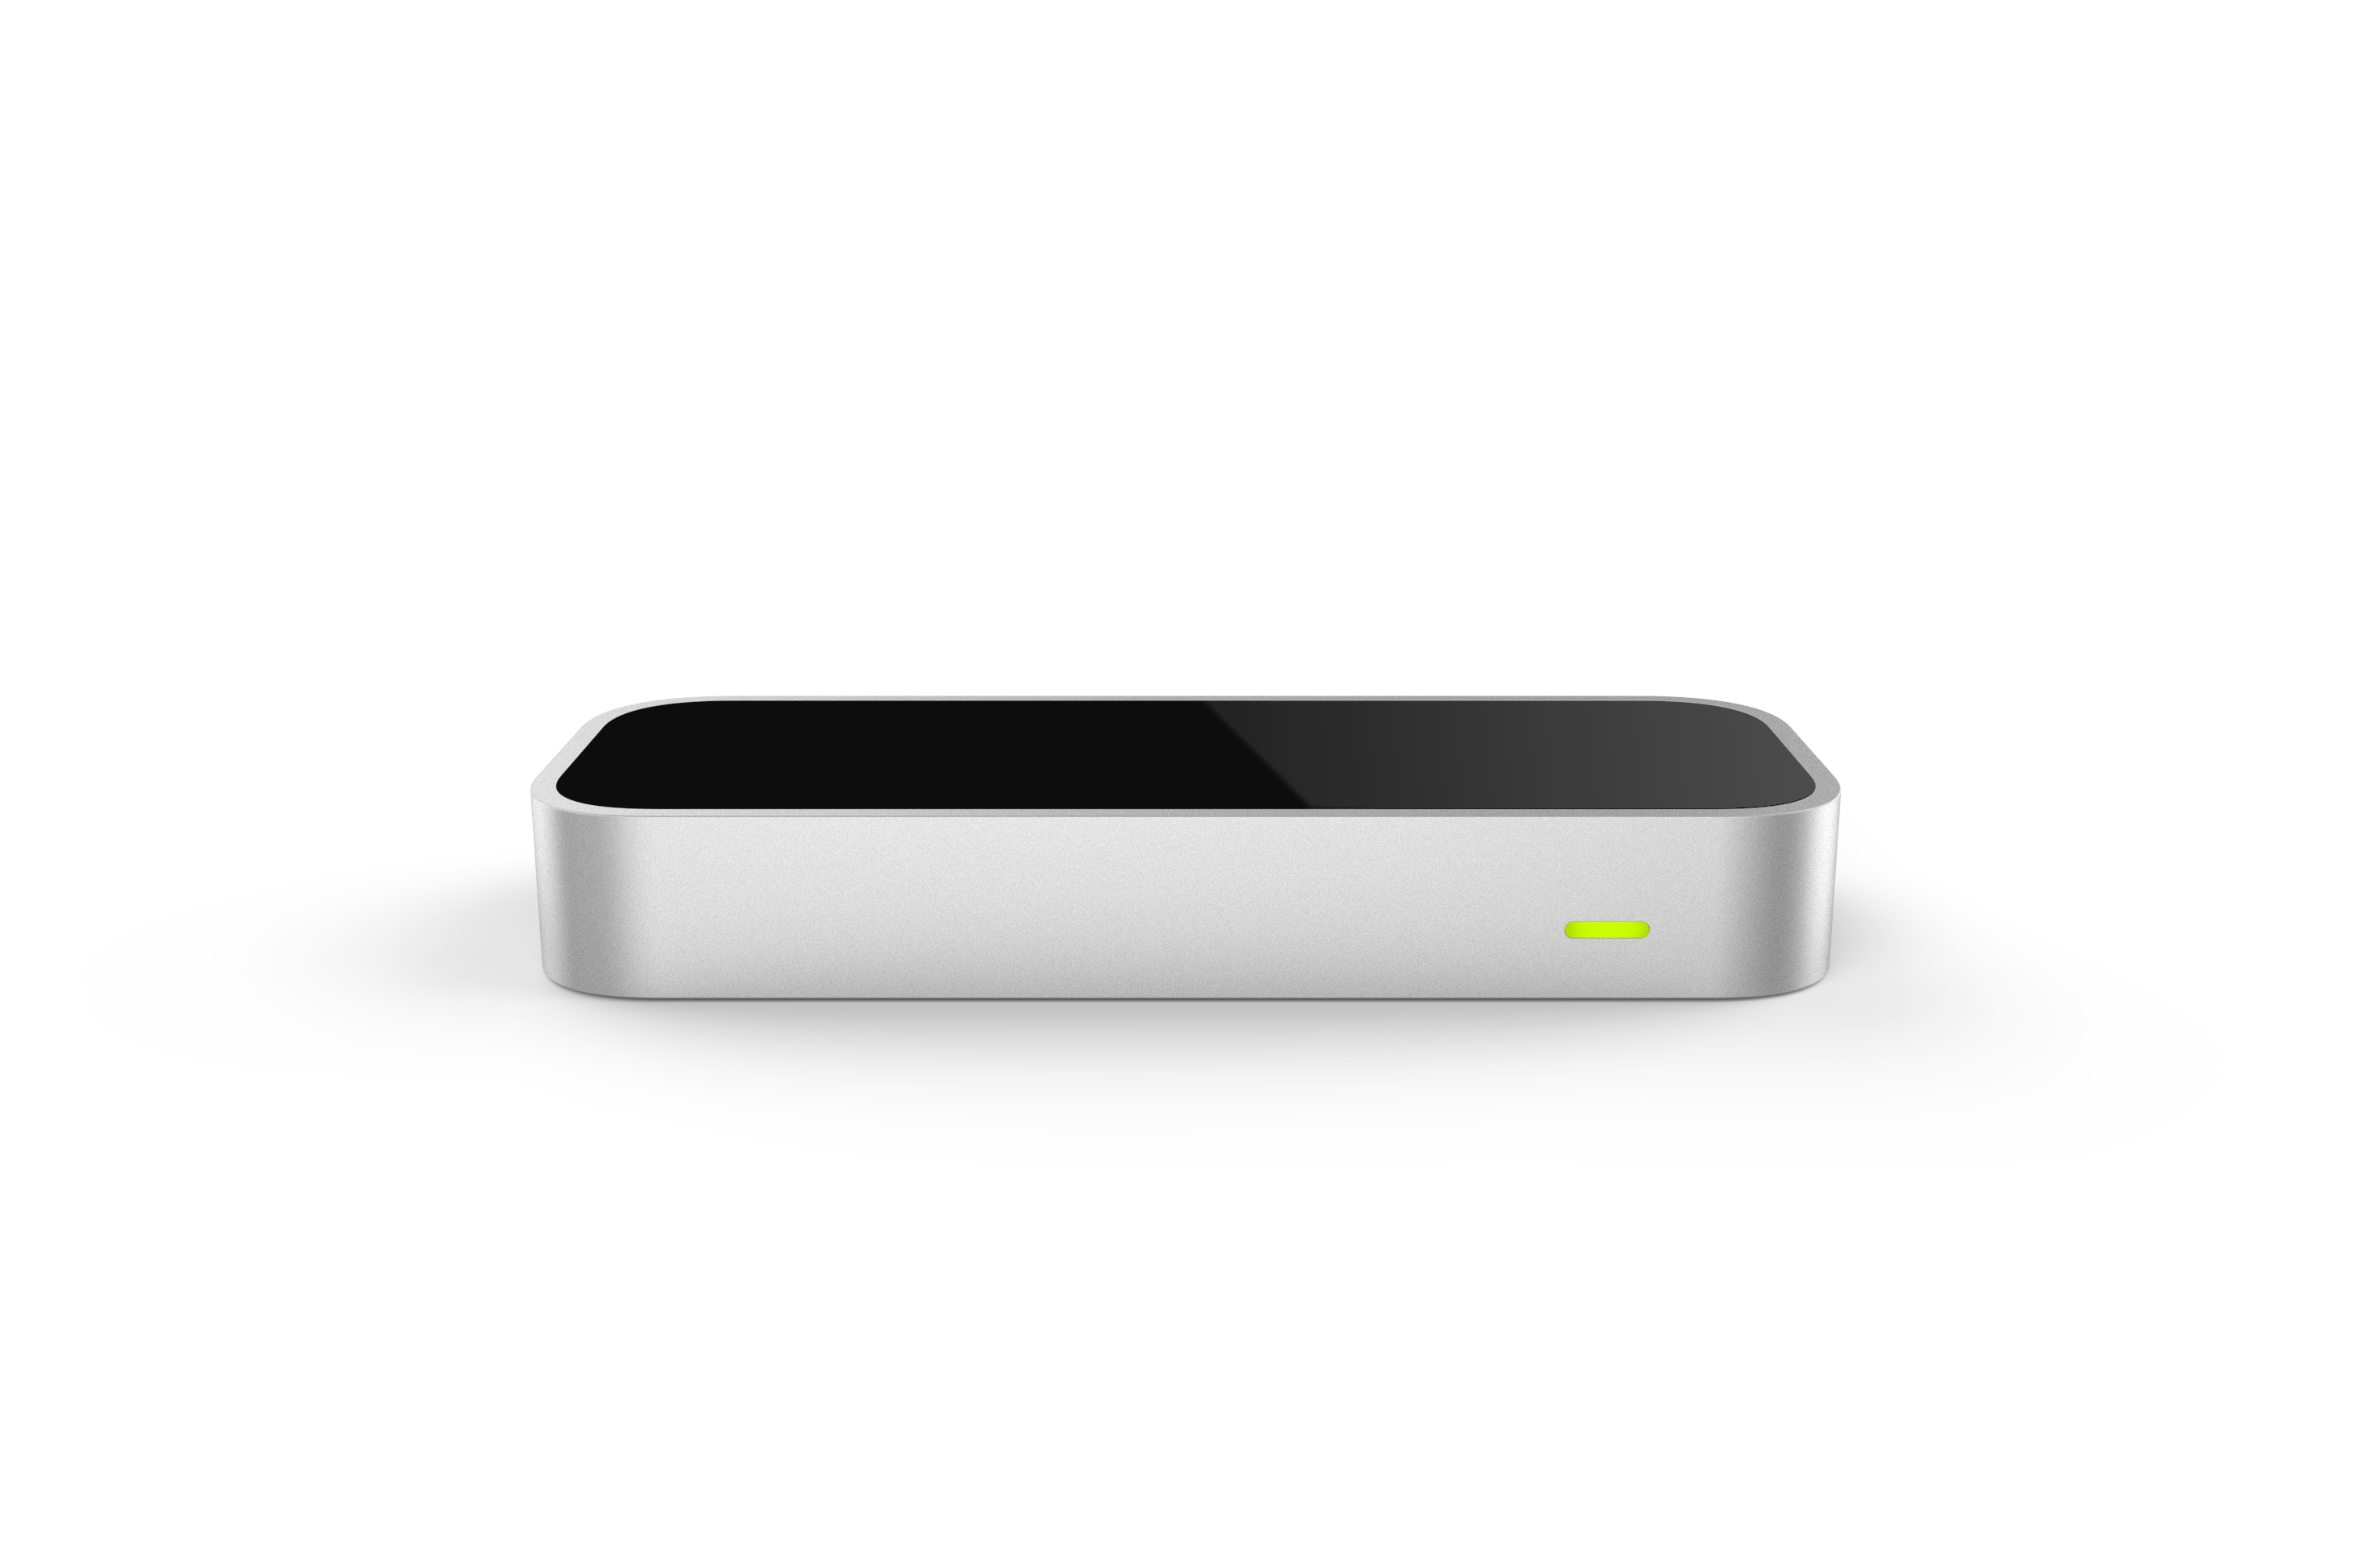
\includegraphics[scale=0.06]{img/LeapMotion.png}
  \caption{dispozitiv Leap Motion}
\end{figure}

Leap Motion este produs de compania americană cu același nume și este un dispozitiv periferic ce poate fi plasat pe o suprafață plată cu fața în sus, sau montat pe parte din față a căștii VR. Folosește două camere cu infraroșu și trei LED-uri infraroșu pentru a observa o zonă aproape semisferică cu raza de aproximativ un metru. LED-urile produc lumină infraroșu continuă, iar camerele generează aproape 200 cadre pe secunda.
Modul exact în care poziția 3D este sintetizată prin compararea celor două imagini 2D generate de camere, nu a fost dezvăluit de companie. Un studiu din 2013 arată că media generală a preciziei cu care controlerul captează și transpune mâinile în obiecte virtuale este de 0,7 milimetri.

\begin{figure}[h]
  \centering
  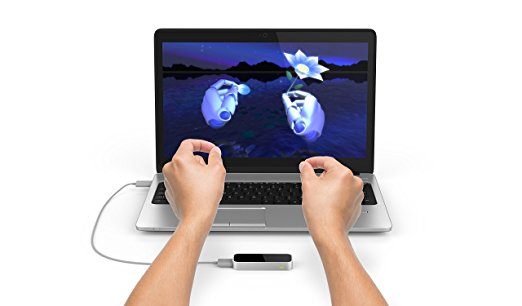
\includegraphics[scale=0.4]{img/leapUse.jpg}
  \caption{dispozitiv Leap Motion în acțiune}
\end{figure}

\section{Unreal Engine}

Un \textit{motor grafic} este un sistem conceput pentru crearea și dezvoltarea de jocuri video. Există mai multe motoare de joc, care sunt proiectate să funcționeze pe console de jocuri video și calculatoare personale. Funcționalitatea de bază oferită de obicei de un motor grafic include un motor de randare\footnote{Din englezescul \textit{renderer}, este rezultatul procesului de preluare și de convertire în imagini a informațiilor digitale introduse într-un mediu programabil de modelare 3D.} pentru grafică 2D sau 3D, un motor de fizică sau de detectare a coliziunilor (și răspunsul la coliziune), sunet, scripting, animație, inteligență artificială, în rețea, streaming, management de memorie, suport de localizare etc. 

\textit{Unreal Engine} este unul din cele mai populare motoare grafice alături de Unity3D, CryEngine, HeroEngine, Rage Engine ș.a.
Dezvoltat de Epic Games, a fost folosit inițial pentru jocul \textit{Unreal} din 1998. Deși conceput pentru jocuri de tip \textit{first-person shooter}\footnote{Tradus \textit{ad litteram} prin \textit{trăgător la prima persoană}, este un gen de joc video în care acțiunea este văzută prin ochii protagonistului.}, este folosit cu succes într-o mare varietate de genuri, printre care \textit{stealth}, \textit{MMORPG-uri}\footnote{\textit{MMORPG}(Massively multiplayer online role-playing game) este o subcategorie a stilului \textit{RPG} (role-playing game) în care jucătorul controlează un personaj inițial slab, dar care pe parcursul poveștii capătă numeroase abilități și în cele mai multe cazuri în funcție de deciziile jucătorului ajunge erou sau antierou, adițional față de RPG, MMORPG-ul este jucat online iar jucătorii pot interacționa atât cu mediul înconjurător cât și între ei.} și alte \textit{RPG-uri}. 

În momentul actual Unreal Engine a ajuns la versiunea 4, care, spre deosebire de versiunile precedente ce rulau cod scris într-un limbaj specific numit \textit{UnrealScript} sau \textit{UScript}, suportă atât programarea în \textit{C++} cât și un sistem de programare vizuală numit \textit{Blueprints Visual Scripting}.

\begin{figure}[h]
  \centering
  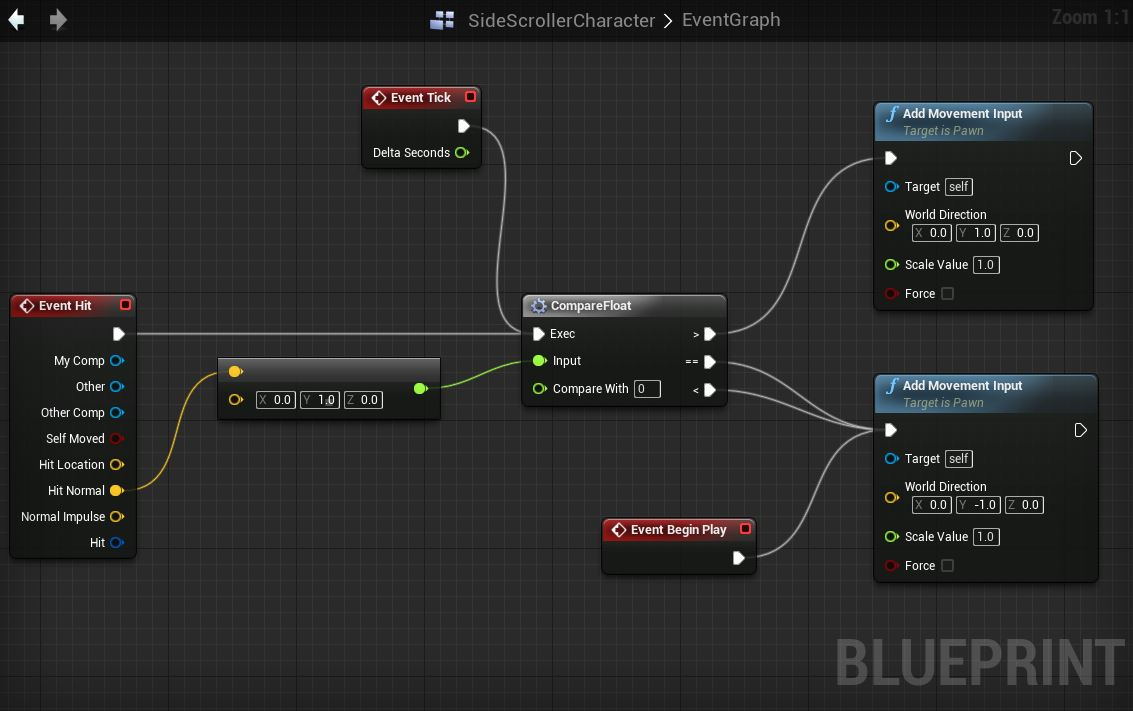
\includegraphics[scale=0.45]{img/simpleBPexample.jpg}
  \caption{Exemplu de script blueprint}
\end{figure}
\newpage